\documentclass[11pt, a4paper, twoside]{article}   	% use "amsart" instead of "article" for AMSLaTeX format

\usepackage{geometry}                		% See geometry.pdf to learn the layout options. There are lots.
\usepackage{pdfpages}
\usepackage{caption}
\usepackage{minted}
\usepackage[german]{babel}			% this end the next are needed for german umlaute
\usepackage[utf8]{inputenc}
\usepackage{color}
\usepackage{graphicx}
\usepackage{titlesec}
\usepackage{fancyhdr}
\usepackage{lastpage}
\usepackage{hyperref}
\usepackage[autostyle=false, style=english]{csquotes}
\usepackage{mathtools}
\usepackage{tabularx}
% http://www.artofproblemsolving.com/wiki/index.php/LaTeX:Symbols#Operators
% =============================================
% Layout & Colors
% =============================================
\geometry{
   a4paper,
   total={210mm,297mm},
   left=20mm,
   right=20mm,
   top=20mm,
   bottom=30mm
 }	

\definecolor{myred}{rgb}{0.8,0,0}
\definecolor{mygreen}{rgb}{0,0.6,0}
\definecolor{mygray}{rgb}{0.5,0.5,0.5}
\definecolor{mymauve}{rgb}{0.58,0,0.82}

\setcounter{secnumdepth}{4}


% the default java directory structure and the main packages
\newcommand{\srcDir}{../src/SolutionUebung2/BoostSpirit}
\newcommand{\imageDir}{images}
% =============================================
% Code Settings
% =============================================
\newenvironment{code}{\captionsetup{type=listing}}{}
\newmintedfile[cppSourceFile]{cpp}{
	linenos=true, 
	frame=single, 
	breaklines=true, 
	tabsize=2,
	numbersep=5pt,
	xleftmargin=10pt,
	baselinestretch=1,
	fontsize=\footnotesize
}
\newmintedfile[jsonFile]{json}{
	linenos=true, 
	frame=single, 
	breaklines=true, 
	tabsize=2,
	numbersep=5pt,
	xleftmargin=10pt,
	baselinestretch=1,
	fontsize=\footnotesize
}
\newmintinline[inlineCpp]{cpp}{}
\newminted[cppSource]{cpp}{
	breaklines=true, 
	tabsize=2,
	autogobble=true,
	breakautoindent=false
}

\newcommand{\xvdash}[1]{%
  \vdash^{\mkern-10mu\scriptscriptstyle\rule[-.9ex]{0pt}{0pt}#1}%
}

% =============================================
% Page Style, Footers & Headers, Title
% =============================================
\title{Übung 3}
\author{Thomas Herzog}

\lhead{Übung 3}
\chead{}
\rhead{
\includegraphics[scale=0.10]{FHO_Logo_Students.jpg}}

\lfoot{S1610454013}
\cfoot{}
\rfoot{ \thepage / \pageref{LastPage} }
\renewcommand{\footrulewidth}{0.4pt}
% =============================================
% D O C U M E N T     C O N T E N T
% =============================================
% =============================================
% 2016.10.13: 1 
% 2016.10.14: 2
% =============================================
\pagestyle{fancy}
\begin{document}
\setlength{\headheight}{15mm}
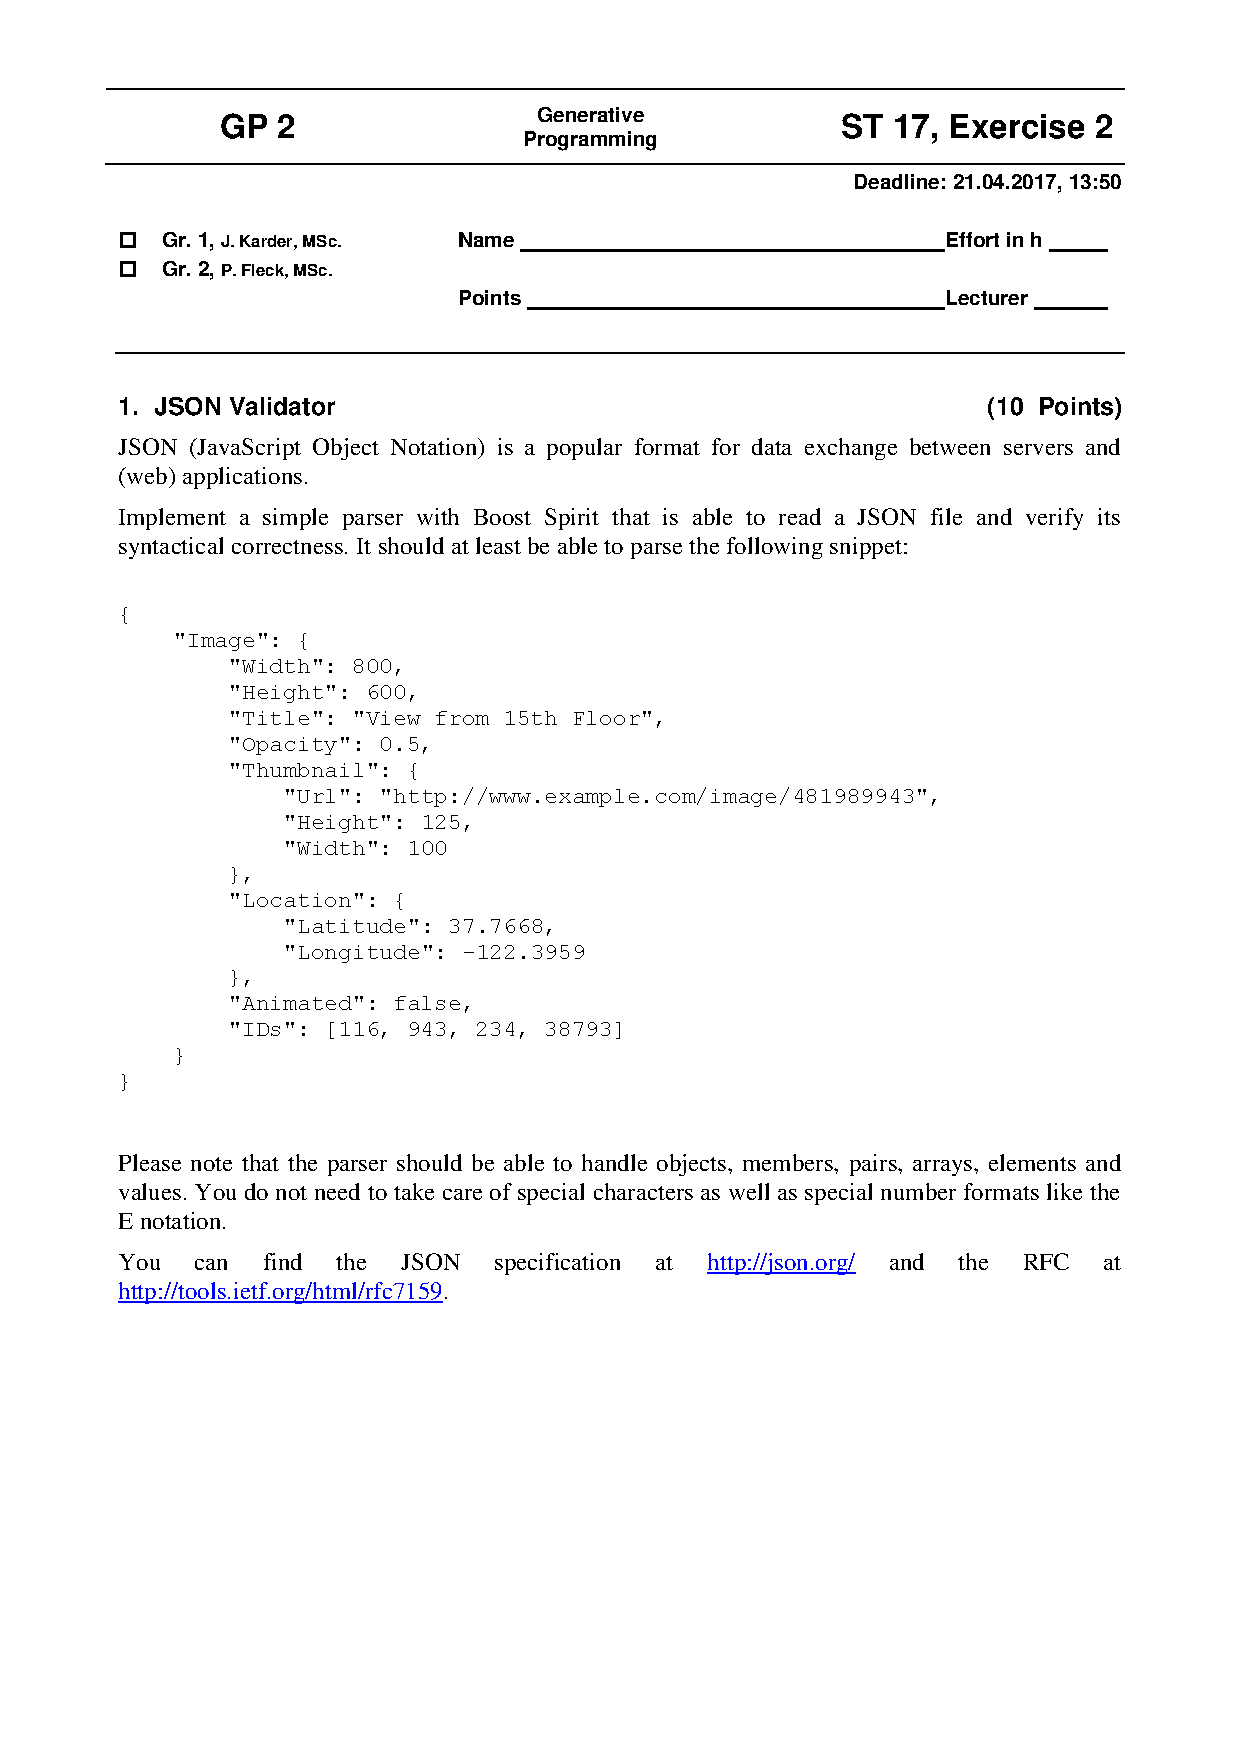
\includepdf[pages={1,2}]{GP_A02.pdf}

\section{JSON Validator}
\subsection{Lösungsidee}
Der \emph{JSON}-Validierer wurde in der \emph{Header}-Datei \emph{json.hpp} implementiert. Die Grammatik wurde gemäß der Grammatik wie auf der Webseite \url{http://json.org} gezeigt implementiert.

\subsubsection{Source}
\begin{code}
	\caption{json.hpp}
	\cppSourceFile{\srcDir/json.hpp}
	\label{src:json-hhp}
\end{code}

\begin{code}
	\caption{test.json}
	\jsonFile{\srcDir/test.json}
	\label{src:json-test}
\end{code}

\begin{code}
	\caption{json-test.hpp}
	\cppSourceFile{\srcDir/json-test.hpp}
	\label{src:json-test-hhp}
\end{code}

\begin{figure}[h]
	\centering
	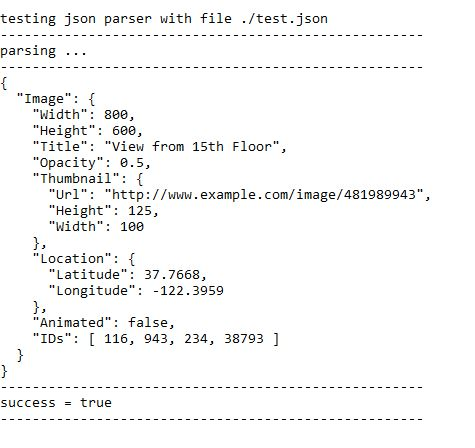
\includegraphics[scale=1]{\imageDir/json.JPG}
	\caption{Test JSON Parser}
	\label{fig:json-4}
\end{figure}
\ \newpage

\subsection{Mini-LOLCODE with Boost.Spirit}
Der Parser mit semantischen Aktionen für die Programmiersprache \emph{LOLCODE} wurde in der \emph{Header}-Datei \emph{lolcode.hpp} implementiert. Es wurden die beiden Datentypen \emph{Numeric} und \emph{Bool} implementiert, wobei auch der Datentyp \emph{Bool} als \emph{Numeric}-Datentyp während des Parsens behandelt wird, also \emph{0=FAIL} und \emph{1=WIN}. Variablen werden in einem assoziativen \emph{Container (map$<$string, double$>$)} gespeichert. Ein zweiter assoziativer \emph{Container (map$<$string, bool$>$)} speichert die Information, ob die Variable ein \emph{Numeric} Datentyp ist oder ob es wich um einen \emph{Bool} Datentyp handelt.
\newline
\newline
Boolsche und arithmetische Ausdrücke können verschachtelt werden, sowie Variablen in den Ausdrücken verwendet werden. Folgende Ausdrücke sind gültig:
\begin{itemize}
	\item\emph{BIGGR OF WIN AN SMALLR OF WIN AN FAIL}
	\item\emph{BIGGR OF 10 AN QUOSHUNT OF 90 AN 10}
	\item\emph{SUM OF 100 AN PRODUKT OF 50 AN num1}
	\item\emph{BOTH SAEM bool1 AN DIFFRINT 100 AN num1}
\end{itemize}
\ \newline
Da auch boolsche Variablen als numerische behandelt werden, sind auch boolsche Variablen in arithmetischen Ausdrücken erlaubt und umgekehrt. Wen in einem boolschen Ausdruck eine Variable eines \emph{Bool}-Datentyp mit einem \emph{Numeric}-Datentypen verglichen werden, so wird die numerische Repräsentation der boolschen variable im boolschen Ausdruck verwendet.
\newline
\newline
Es wurden alle \emph{String}-Konstanten wie z.B. \emph{VISIBLE} als \emph{boost spirit} Literale in der Grammatik definiert \emph{(qi::lit("VISIBLE"))} und nicht als \emph{String} angegeben.
 
\subsubsection{Source}
\begin{code}
	\caption{lolcode.hpp}
	\cppSourceFile{\srcDir/lolcode.hpp}
	\label{src:lolcode-hhp}
\end{code}

\VerbatimInput{\srcDir/test.lolcode}

\begin{code}
	\caption{lolcode-test.hpp}
	\cppSourceFile{\srcDir/lolcode-test.hpp}
	\label{src:lolcode-test-hhp}
\end{code}

\begin{code}
	\caption{main.cpp}
	\cppSourceFile{\srcDir/main.cpp}
	\label{src:main-cpp}
\end{code}

\begin{figure}[h]
	\centering
	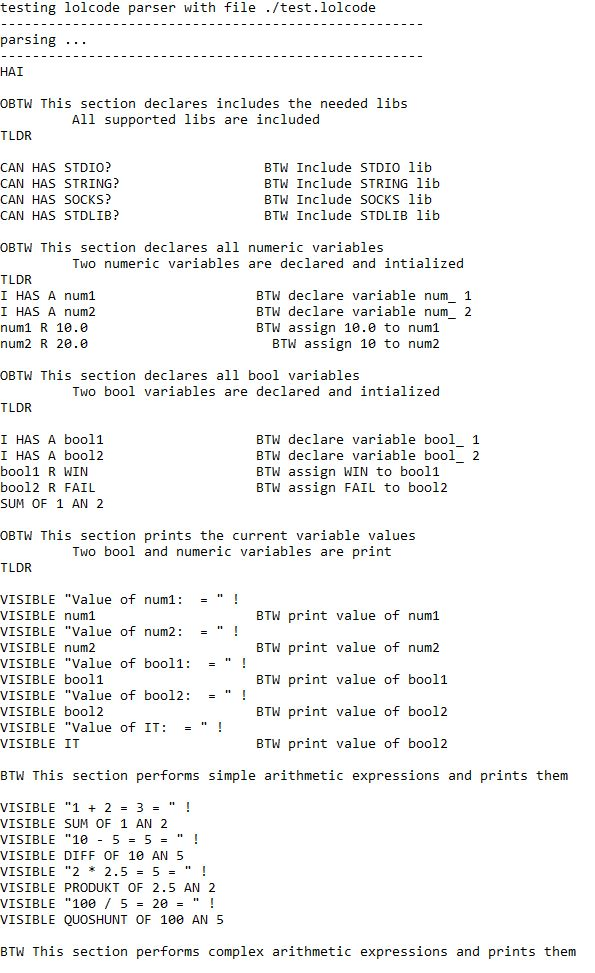
\includegraphics[scale=0.9]{\imageDir/lolcode-1.JPG}
	\caption{Test Teil 1}
	\label{fig:lolcode-1}
\end{figure}

\begin{figure}[h]
	\centering
	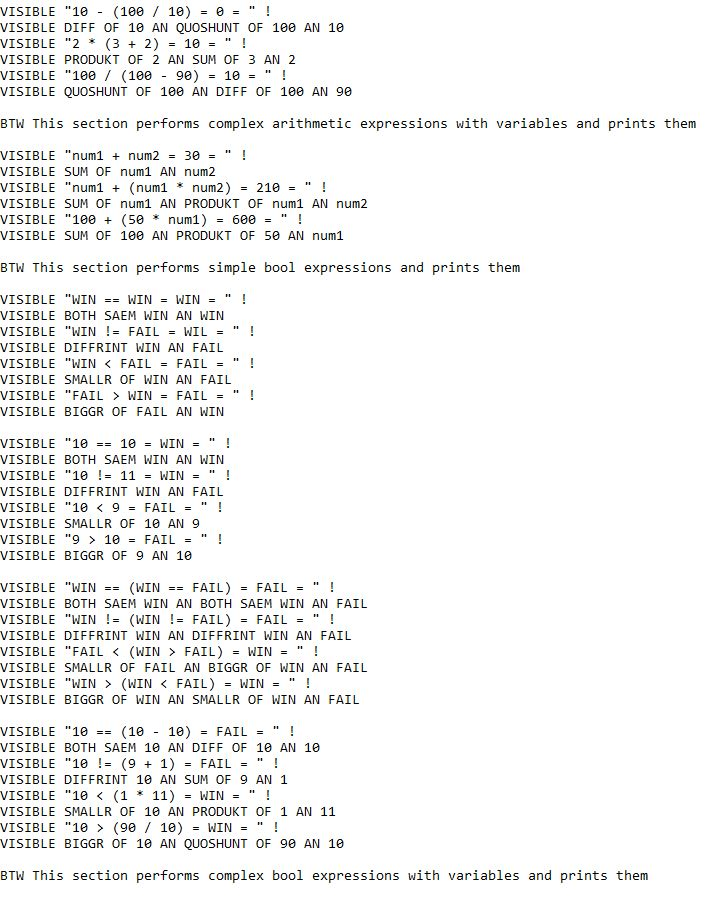
\includegraphics[scale=0.9]{\imageDir/lolcode-2.JPG}
	\caption{Test Teil 2}
	\label{fig:lolcode-2}
\end{figure}

\begin{figure}[h]
	\centering
	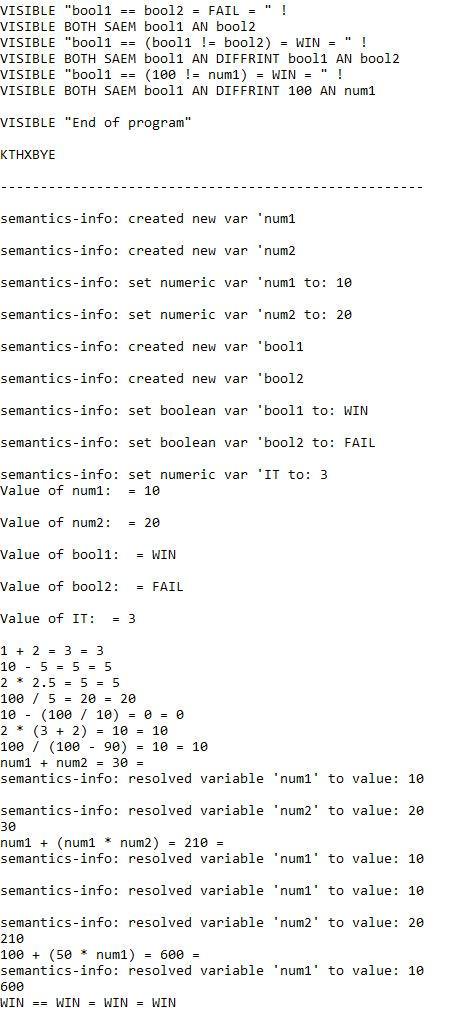
\includegraphics[scale=0.9]{\imageDir/lolcode-3.JPG}
	\caption{Test Teil 3}
	\label{fig:lolcode-3}
\end{figure}

\begin{figure}[h]
	\centering
	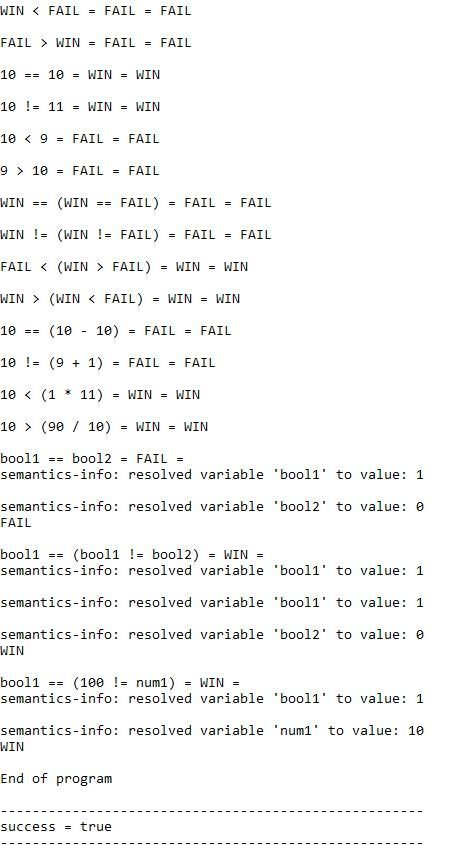
\includegraphics[scale=0.9]{\imageDir/lolcode-4.JPG}
	\caption{Test Teil 4}
	\label{fig:lolcode-4}
\end{figure}

\end{document}